\documentclass[a4paper]{article}

%\usepackage{fullpage} % Package to use full page
\usepackage{parskip} % Package to tweak paragraph skipping
\usepackage{tikz} % Package for drawing
\usepackage{amsmath}
\usepackage{hyperref}
\usepackage[T1]{fontenc}
\usepackage[utf8]{inputenc}
\usepackage[french]{babel}
\usepackage{wrapfig}

\title{Semaine du 06/08}
\author{Reda YAHOU}
\date{\today}

\begin{document}

\maketitle

\section*{Introduction}

Ce document a pour but de résumer le travail qui a été réalisé durant la semaine du 07/08. Ce papier a pour but de proposer un algorithme afin de modéliser la trajectoire et la stabilité des fusées pour le cas bi-étagées.\\




\begin{figure}[!htbp]
\begin{center}
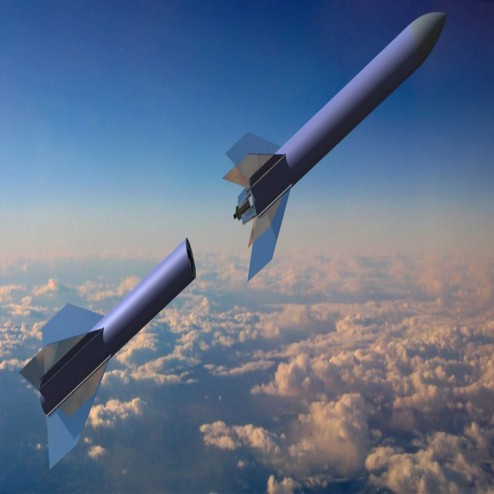
\includegraphics[width=6cm]{complet-1024x494.jpg} 
\end{center}
\caption{Fusée bi-étage.}
\end{figure}





\section{Vol des fusées bi-étagée}

L'interface Pégase ne réalise les calculs que pour les fusées mono étagées. Le cas des fusées multi-étagée est un peu différent dans la mesure ou il fait entrer d'autres paramètres en jeu : \\

\begin{itemize}
\item La fusée se sépare de ses étages à un moment donnée, entrainant un changement de masse et de géométrie.
\item Il faut par la suite considérer la stabilité et la trajectoire de chaque étage de la fusée indépendamment.
\end{itemize}

En résumé le vol se déroule en trois phases : 

\begin{enumerate}

\item Vol en configuration bi-étage entre $t_{0}$\footnote{instant initial} et $t_{1}$\footnote{instant de séparation},
\item Vol du premier étage seul indépendamment,
\item Vol du deuxième étage seul indépendamment

\end{enumerate}

Les changements de masse et de géométrie vont avoir un impact direct sur les forces mise en jeu et donc sur le schéma numérique modélisant la trajectoire.


\section{Schéma numérique}

\begin{verbatim}

M_0,i, M_1,i, M_2,i \\la masse total de la fusée, de l'étage 1 et 2 à ti

dm1,i, dm2,i \\ débit massique de l'étage 1 et de l'étage 2


\end{verbatim}




\section{Conclusions}

Durant les prochains jours, on va tenter de formaliser la modélisation des fusée bi-étagée et l'étude de leur stabilité et trajectoire et enfin, d'inclure cela à l'interface de calcul Pégase.


%\bibliographystyle{plain}
%\bibliography{bibliography.bib}
\end{document}
